% Paper for the ChouchBase assignment.

\documentclass[]{IEEEtran}

\usepackage{float}
\usepackage{url}
\usepackage{graphicx}
\usepackage{color}

\begin{document}

\title{No Dogs On The Couch$_{Base}$}

% author names and affiliations
% use a multiple column layout for up to two different
% affiliations

\author{\IEEEauthorblockN{Eriq Augustine, Ryan Hnarkis, Aldrin Montana, Ryan Verdon, Tyler Yero}
\\
\IEEEauthorblockA{Department of Computer Science\\
Cal Poly, San Luis Obispo\\
 \textsf{\{eaugusti, rhnaraki, amontana, rverdon, tyero\}@calpoly.edu}
}
}

\maketitle

\thispagestyle{empty}
\pagestyle{empty}

\section{Introduction}
Our team decided to compare a MySQL cluster versus a Couchbase cluster for running a
web application. We are using an eight table SQL schema from Ryan Verdon's Thesis. To evaluate
the performance we autogenerated around 400MB of data and inserted the same data into each cluster.
Obviously using a different data model for Couchbase to accomodate for the fact it is a NoSQL key-value store
instead of a relational database. We then created a set of six experiments to run. Five came from common 
use cases found in the web application. While the other was designed to test the performance on each cluster
of repeatedly writing and reading from the same object. Our major metrics are write performance, read performance,
and time-delay between writes and reads of the same data. The rest of the paper is broken down as follows.
Section 2 describes in depth how we designed the experiment. Section 3 discusses the workloads we ran on each system. Section 4 describes our implementation. Section 5 goes
into the results of each of our experiments and some analysis on the data we obtained. Lastly, section 6 presents 
our conclusions.

\section{Experiment Design}
For our experiments we are using a total of five EC2 instances from the Amazon Web Services cloud. For both of our systems four servers were used for the database while the last was used for running our workload harness. The MySQL system is setup with one master server for writes and three slaves servers that replicate all of the masters data. Unlike the Couchbase system where we had four servers setup for reads and writes of the keys they were incharge of.

Our major driving force of this experiment was to see how Couchbase compared to MySQL for running a web application. To test which is better we created a workload harness. The main task of the workload harness was to define how many times a workload would run. In our case workloads define a certain task. For example, getting of the data necessary to display a users profile. We leave describing each workload we ran to the next section. Here we will focus on the design of the systems. 

As each workload is run the workload harness records important stats. Some of the stats include how long the workload took to run, the min and max times of an individual query or insertion, and the standard deviations of individual runs.

\subsection{Data}
The data we are storing comes from Ryan Verdon's masters thesis. It is the backend for a community genome annotation database. So it has data like genome sequences, genes, and species information. The representation of the data is vastly different in the two systems. There exists four main pieces of data that are cruicial to either representation. They are Contigs, Annotations, Users, and Groups. Contigs are what a biologist annotates which basically means looks at to find a gene. The main portion of a contig is a DNA sequence. Annotations are the record or formal representation of a gene that has been found in a contig. An annotation has several parts. The main ones are coordinates in the contig of where individual exons are located and a ton of meta information about the annotation like who uploaded it and when it was done, etc. Users is an important part of the data it is one of the central pillars that connects the data. Users upload contigs, create annotations, and join groups. Groups are an important part of the usefulness of the system. Users of likemindness can join the same group to receive important information that is important to them. Below we discuss the different ways we store the data in SQL versus JSON.

\subsubsection{SQL}
The relational schema for the MySQL cluster is shown in Figure~\ref{fig:SQLDiagram}.

\subsubsection{JSON}
The JSON objects for the Couchbase cluster are shown in Figure~\ref{fig:JSON}.

\clearpage
\begin{figure}%
{%
\setlength{\fboxsep}{0pt}%
\setlength{\fboxrule}{1pt}%
\fbox{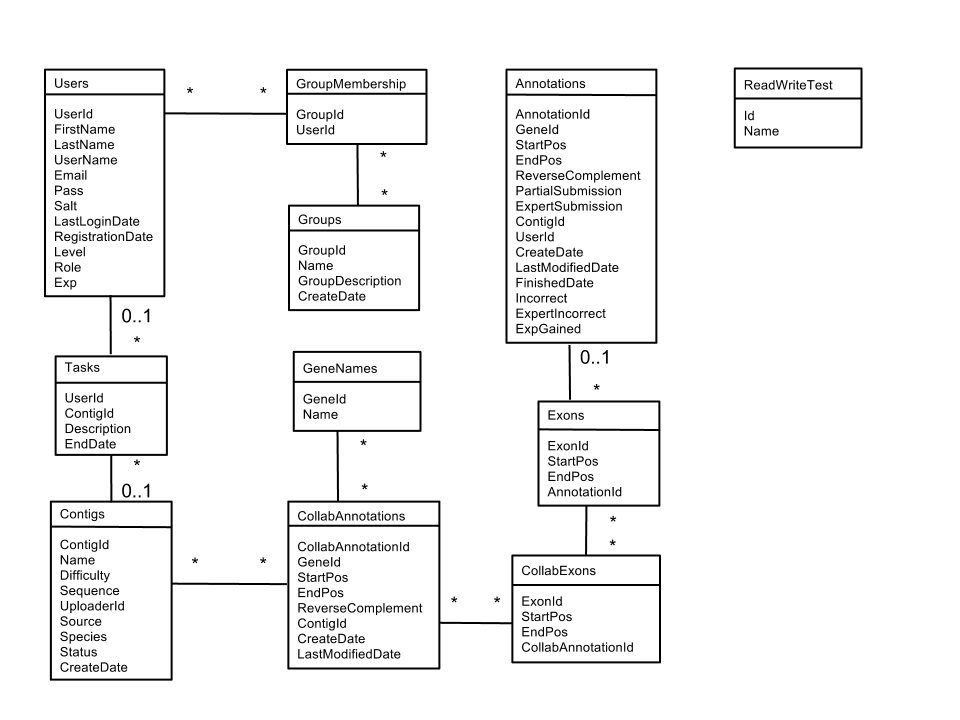
\includegraphics[width=180mm]{SQLDiagram.png}}%
}%
\caption{The SQL Schema for CGAT.}
\label{fig:SQLDiagram}
\end{figure}%

\clearpage
\begin{figure}%
{%
\setlength{\fboxsep}{0pt}%
\setlength{\fboxrule}{1pt}%
\fbox{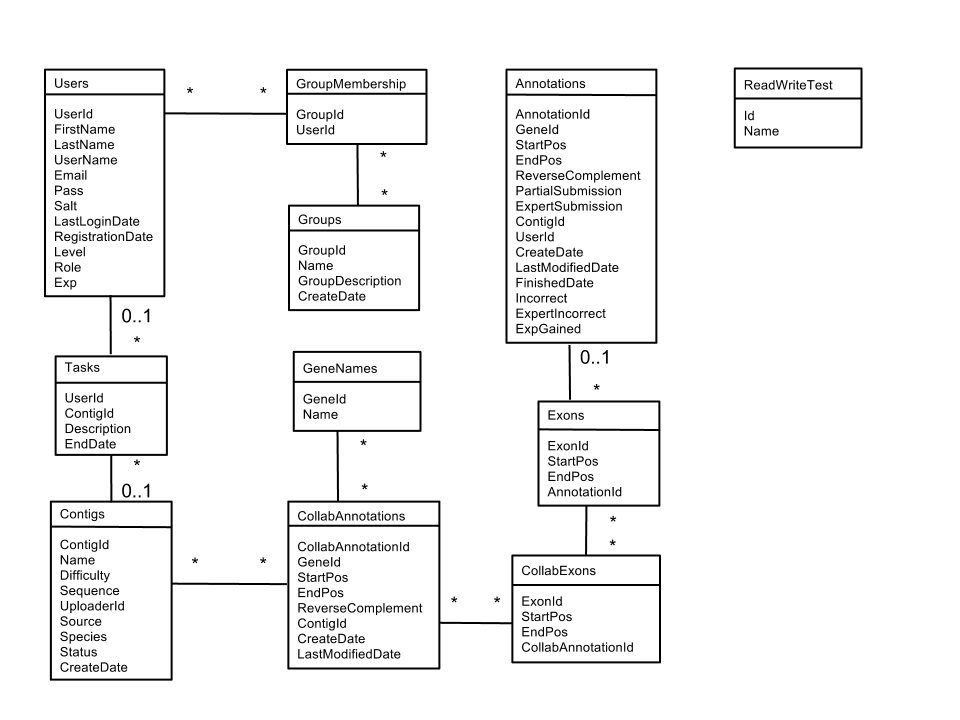
\includegraphics[width=180mm]{SQLDiagram.png}}%
}%
\caption{The JSON object definitions for CGAT.}
\label{fig:JSON}
\end{figure}%

\clearpage
\section{Workloads}
The following workloads were ran on both the MySQL and Couchbase clusters.
\subsection{Assigning a Task}
This workload comes from a use-case in the web application. The main idea is that a new contig has been uploaded and some users that care about this contig need to be notified. 

\subsection{Profiling}
The profiling workload simulates what happens when all of the information about a user is gathered. This includes: all groups they are a member of, all full and partial annotations they have submitted, and all tasks they have assigned. This is a read-heavy workload.

\subsection{Publishing}
This workload involves updating a user's experience because of a completed annotation. The corresponding annontation record must also be set to complete, have its finished date updated, and have its gained experience set. This is a write-heavy workload.

\subsection{Adding and Removing Group Membership}
Adding or removing users to a group is a task common for classroom situations. In MySQL, this operation requires a join between three tables: Groups, Users, and GroupMembership. In Couchbase, this requires retrieving the key for the desired group and removing the user from the members field. This is a mixed workload involving reading and writing.

\subsection{Uploading Contigs}
This workload represents a contig being inserted into the database. All of the attributes of a contig are set, including the user who uploaded it and its sequence. This is a write-heavy workload.

\subsection{Read and Writing Performance}
TODO

\section{Implementation}
Our experiment was implemented completly in Java. To do the MySQL portion of the workload we used
the MySQL JDBC driver. For the Couchbase portion we used their Java library from their website.

\section{Evaluation}
TODO

\section{Conclusions}
TODO

% TODO: Uncomment if we use any refs
% \bibliographystyle{acm}
% \bibliography{refs}

\end{document}
